\documentclass[10pt]{article}
\usepackage[letterpaper,margin=0.75in]{geometry}
\usepackage[T1]{fontenc}
\usepackage{lmodern,microtype,graphicx,booktabs,amsmath,enumitem,needspace}
\usepackage[hidelinks]{hyperref}
\makeatletter\long\def\@makecaption#1#2{\vskip3pt{\small\textbf{#1.} #2\par}}\makeatother
\setlength{\parindent}{0pt}\setlength{\parskip}{4pt}
\setlist{nosep,leftmargin=*}
\newcommand{\mysec}[1]{\needspace{5\baselineskip}\vspace{5pt}{\large\bfseries #1\par}\vspace{1pt}}
\makeatletter\renewcommand{\section}{\@ifstar\mysec\mysec}\makeatother
\newcommand{\sub}[1]{\textbf{#1}\ }
\pagestyle{plain}

\begin{document}
{\Large\bfseries Does forecasting AI model releases first improve forecasts of small-business AI use?}\\[2pt]
ISYE 4031 Milestone 3 \textbullet{} Group 1 \textbullet{} November 22, 2026\\
Rahul Mehta, Ishaan Mohan, Zhengyu Chris Liu, Timothy Kim, Chau M Duong

\section{1. Question and motivation}
\sub{What we set out to discover.} Milestone 2 forecast an industry-by-size group's AI-use rate (Census BTOS, employers with 1--99 employees) three releases, about six weeks, ahead. A ridge regression on current use, history, industry, size and trend beat a six-release average at every issue date. One idea kept coming up: new AI models come out in bursts, and those bursts might drive adoption. So we asked a direct question. \emph{If we first forecast how many AI models will be released, and feed that forecast into the adoption model, do adoption forecasts get better?}

\sub{Why it matters.} A support organization planning AI outreach would like to know whether to watch the model-release calendar. If a two-stage model helps, release forecasts are worth maintaining. If not, the simpler model is enough.

\sub{What motivated it.} At Milestone 2 the professor suggested modeling release timing with a nonstationary Poisson process. At the Milestone 3 check-in he asked us to (i) compare direct and two-stage forecasting on the same observations, (ii) explain \emph{why} they differ, since a more complex model is not automatically better, (iii) justify the Poisson model and interpret its error against baselines, (iv) add variables only when they clearly help, and (v) end with a conclusion backed by evidence. This report is organized around those requests.

\sub{Expectation.} We expected release forecasts to help only if releases change adoption within six weeks and if stage 1 forecasts them well. Evidence against would be no gain even when stage 1 is given the actual release counts.

\section{2. Method and experiment}
\sub{Stage 1: release counts.} Data are the Epoch AI scored-model catalog frozen on October 30, 2026: 221 releases since January 2024, forming 179 provider-day batches. Releases are counts of separate events whose rate grows over time, so we model daily arrivals as a nonhomogeneous Poisson process,
\[
Y_d\sim\operatorname{Poisson}(\lambda_d),\qquad \log\lambda_d=\beta_0+\beta_1 t_d+\beta_2 W_d,
\]
with $t_d$ years since January 2024 and $W_d$ a weekday indicator. The log link keeps the rate positive and lets it grow by a fixed percent per year. Linear regression would allow negative counts and assume constant variance, while a Poisson count's variance equals its mean. Providers often release several models on one day, which breaks independence. Following the batch-arrival formulation in \cite{compound}, we also fit a compound Poisson model: batches arrive as $B_d\sim\operatorname{Poisson}(\nu_d)$ and each batch holds $K\ge1$ models, so $E(Y_d)=\nu_dE(K)$ and $\operatorname{Var}(Y_d)=\nu_dE(K^2)$. Each model is refit at each issue date on releases published by then. The stage-1 output is the expected number of releases in the 24 days from the issue date to the target survey's reference date.

\sub{Data.} Adoption data are the Census BTOS sector-by-size workbook (October 20, 2026), 23 releases from the November 2025 question revision to October 8, 2026. Suppressed cells (22.6\%) stay missing, and we keep 71 groups with enough history. One observation is a group in one biweekly release, not a firm, so the target is a published survey estimate with its own standard error.

\sub{Stage 2: adoption.} Every arm uses the same 706 forecasts for 71 groups (15 industries, five size bands) at 10 issue dates (April 23 to August 27, 2026), the same expanding window, and the same ridge penalty chosen by inner time-ordered folds. Preprocessing is fit on training data only, and a training pair enters only after its target was published.
\begin{itemize}
\item \textbf{Direct:} the Milestone 2 control ridge (current rate, lags, industry, size, trend and controls).
\item \textbf{Two-stage:} direct plus the Poisson release forecast. \textbf{Two-stage, batch:} direct plus the compound Poisson forecast.
\item \textbf{Actual-count diagnostic:} direct plus the \emph{actual} release count in the window. This uses future information, so it is not a usable forecast. It asks whether release counts help when stage 1 is perfect.
\end{itemize}
\sub{Metrics and test.} MAE and RMSE in percentage points (pp), MAE by size band, dates won out of 10, and a 95\% moving-block bootstrap interval for the mean date-level MAE difference (3-date blocks; 2 and 4 give the same signs). Stage 1 is scored by count MAE on 22 completed 24-day windows, and in Chris's separate study on six non-overlapping 42-day windows with log loss and 90\% interval coverage.

\section{3. Results and discoveries}
\sub{Two-stage forecasting did not improve adoption forecasts.} Table~1 shows the direct model has the lowest error. Adding predicted releases raised MAE by 0.10 pp and won at only 2 of 10 dates. The batch version did slightly better than plain Poisson but still lost to direct. Most importantly, even the \emph{actual} release counts did not help (+0.04 pp, 4 of 10 dates).

\begin{table}[h]\centering\footnotesize\setlength{\tabcolsep}{4pt}
\begin{tabular}{@{}lrrrrrr@{}}\toprule
Adoption forecast (706 forecasts) & MAE & RMSE & Bias & MAE 1--4 emp. & MAE 50--99 emp. & vs.\ direct, 95\% interval\\\midrule
Carry latest rate forward & 4.15 & 5.75 & $-1.05$ & 2.29 & 6.66 & \\
Six-release mean & 3.39 & 4.64 & $-2.07$ & 2.53 & 4.65 & $+0.25$ [$+0.17$, $+0.35$], 0/10\\
\textbf{Direct ridge} & \textbf{3.14} & \textbf{4.32} & $+0.47$ & \textbf{2.03} & 4.99 & \\
Two-stage, Poisson & 3.24 & 4.41 & $+0.65$ & 2.14 & 4.94 & $+0.10$ [$+0.00$, $+0.27$], 2/10\\
Two-stage, compound Poisson & 3.22 & 4.40 & $+0.61$ & 2.12 & 4.91 & $+0.08$ [$+0.01$, $+0.21$], 3/10\\
Actual release counts (diagnostic) & 3.17 & 4.37 & $+0.54$ & 2.08 & 4.98 & $+0.04$ [$-0.01$, $+0.12$], 4/10\\\bottomrule
\end{tabular}
\caption{Adoption error in percentage points. Last column: mean change in date-level MAE against direct (positive is worse), block-bootstrap interval, and dates where the model beat direct. Ten dates give limited precision, so the intervals are exploratory.}
\end{table}

\sub{The Poisson model forecasts releases reasonably well.} Table~2 interprets stage-1 error against baselines. The average window holds 6.3 releases, so a 2.6-release miss is large in relative terms, but it beats carrying the last count forward (27\% lower error) and the historical average rate (12\% lower). The data are overdispersed (Pearson dispersion 1.37, where 1 is ideal), so plain Poisson intervals are too narrow: the 90\% interval covered only 77\% of windows. Modeling batches fixes much of this. On 42-day windows, the weekday model expects 7.7 days with two or more releases against 16 observed, while the compound model expects 14.4, and count MAE falls from 3.39 to 2.81. A quadratic trend (3.57) and shorter rate histories (4.58 with 365 days) were worse, so added flexibility did not help in stage 1 either.

\begin{table}[h]\centering\small
\begin{tabular}{@{}lrr@{}}\toprule
Release forecast & MAE, 24-day windows (22) & MAE, 42-day windows (6)\\\midrule
Previous window's count & 3.50 & \\
Historical average / constant rate & 2.90 & 4.75\\
Poisson, time + weekday & 2.56 & 3.39\\
Compound Poisson, time + weekday & \textbf{2.44} & \textbf{2.81}\\\bottomrule
\end{tabular}
\caption{Stage-1 count error (releases per window). The 42-day study also scored log loss, interval width and interval score; the compound model was best or tied on all of them.}
\end{table}

\begin{figure}[h]\centering
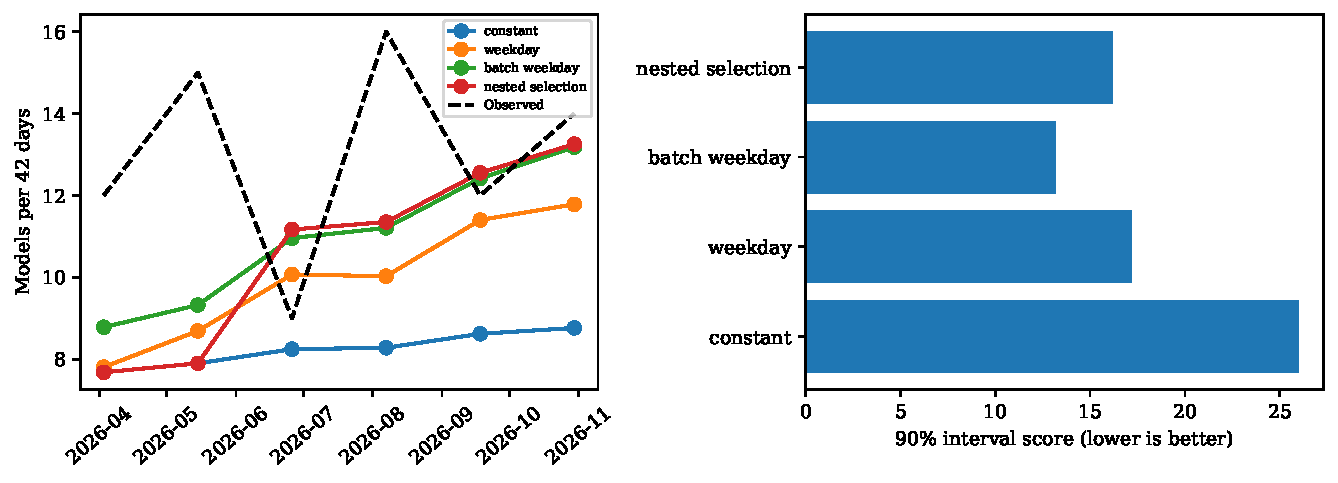
\includegraphics[width=.92\linewidth]{../results/poisson_investigation/comparison.pdf}
\caption{Stage-1 study on six 42-day windows. Left: predicted and observed release totals. Right: interval scores, which penalize both wide intervals and misses. Batch (compound) models score best.}
\end{figure}

\begin{figure}[h]\centering
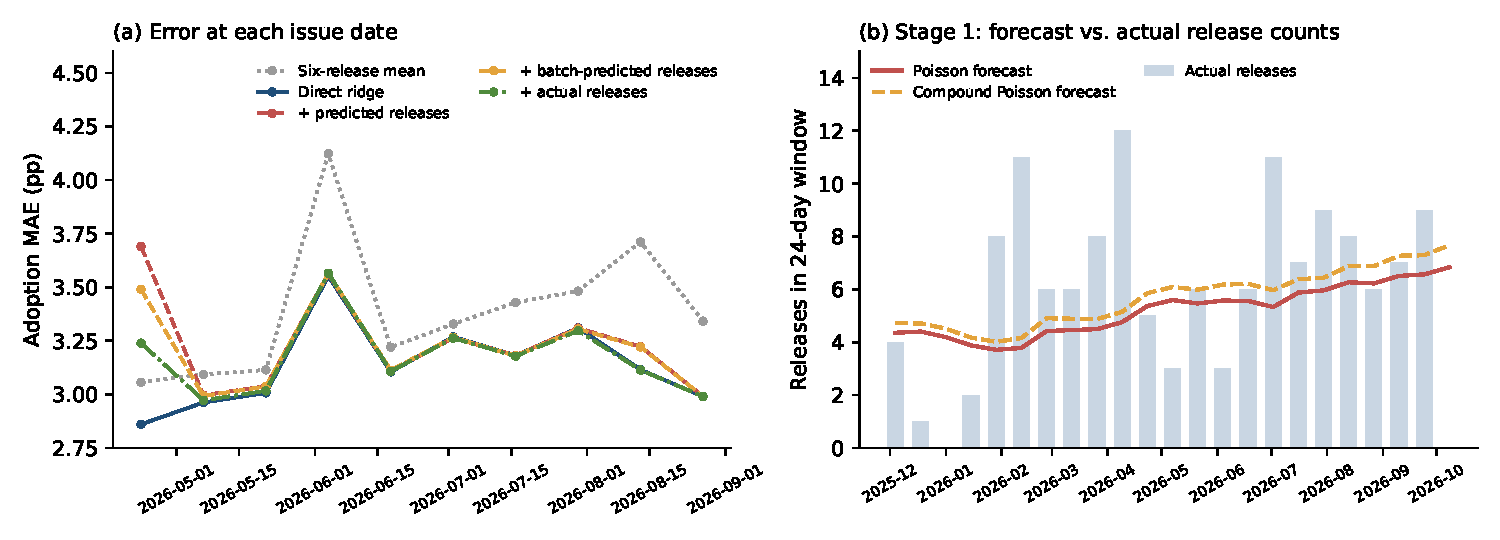
\includegraphics[width=\linewidth]{fig_two_stage.pdf}
\caption{(a) Adoption MAE at each issue date. All release arms track direct except on April 23. (b) The stage-1 forecast is a smooth upward trend, while actual counts swing from 0 to 12.}
\end{figure}

\sub{Why the models perform differently.} We tested four explanations.
\begin{enumerate}
\item \emph{Release counts carry little information for this target (supported).} The release count is one number shared by all 71 groups on a date, so it can only explain movement every group shares, which the trend already captures. Even the actual counts did not help. For this input and model, a better stage 1 has little to offer.
\item \emph{Stage 1 is mostly a time trend (supported).} The Poisson forecast correlates 0.94 with time (VIF 8.2 against the trend term) but only 0.20 with the actual count (Figure 2b). It gets the level right and misses the swings, so it adds a noisier copy of information the model already has.
\item \emph{Stage-1 errors carry into stage 2 (consistent, not isolated).} Predicted counts lost to actual counts at 9 of 10 dates (+0.06 pp, interval [$+0.00$, $+0.15$]). Swapping the input also changes the fitted penalty, so this is not a clean measure of error propagation.
\item \emph{Sensitivity to regularization at one date (supported).} At April 23, tuning chose a weaker penalty for the release arms ($\alpha=100$ vs.\ 1000). The two-stage model fit training data better (MAE 2.88 vs.\ 3.44) but forecast worse (3.69 vs.\ 2.86). Without that date, the two-stage gap shrinks from 0.10 to 0.02 pp. The extra input gave the model room to fit noise in a short early history.
\end{enumerate}
Survey noise also limits all models: 86\% of direct errors are within two survey standard errors of the target, and error for 50--99 employees (about 5 pp) stays high in every arm.

\sub{Where it fails.} The loss is broad, not driven by one group. The two-stage model beat direct in only 3 of 15 industries (best: Construction, $-0.17$ pp) and lost most in Manufacturing ($+0.37$) and Information ($+0.32$), which already has the highest error. It was worse in four of five size bands; only 50--99 employees improved slightly ($-0.05$). Chau's breakdown of the broader benchmark-plus-Poisson model finds the same pattern: it is worse in 13 of 15 industries and all five size bands. So the release signal does not help a particular kind of business that the pooled average hides.

\sub{Additional variables.} Under the same protocol, earlier runs added past 42-day release counts (+0.07 pp vs.\ the ridge control), benchmark capability scores (+0.05), benchmarks plus the Poisson forecast (+0.13), and industry interactions (+0.11); boosting with all of them was a tie ($-0.01$). Expected use was dropped at Milestone 2 for the same reason. We set the rule before looking: keep a variable only if it lowers MAE by more than 0.1 pp and wins at most dates. None passed, so the direct model keeps its original inputs.

\section{4. Reflection}
\sub{What did not improve, and what we tried.} The two-stage model did not beat direct forecasting. We responded by (a) improving stage 1 with batches, which lowered release error but barely changed adoption error, (b) giving stage 2 the actual counts, which showed the input itself is weak, and (c) checking each date, which located most of the loss at one early date with a weak penalty. Tested: the shared-input, trend-overlap and regularization explanations. Conjecture only: that businesses respond to release news on a longer horizon than six weeks.

\sub{Response to check-in feedback.} The professor asked for a fair comparison, reasons, a justified Poisson model, tested variables and an evidence-based conclusion. We answered each: Table~1 compares all arms on identical forecasts; the actual-count diagnostic and per-date checks give the reasons; Table~2 and Figure~1 judge the Poisson error against baselines; the variable rule is stated before results; and Section~4 states what the evidence supports. We also replaced independence-based $p$-values with block intervals, since forecasts at nearby dates share shocks.

\sub{What we learned from the source and feedback.} The compound Poisson source changed our event unit from single models to provider-day batches; we kept time and weekday effects and dropped the quadratic trend. The professor's point that complexity is not accuracy led us to add the actual-count diagnostic, which answered the question more clearly than any extra model would have.

\sub{What we can and cannot conclude.} For this target, horizon and data, the direct model is the more reasonable choice: it is simpler, more accurate, and has no upstream stage that can fail. The Poisson model remains a sound way to forecast releases themselves. We cannot conclude that AI releases do not affect adoption, only that release counts do not improve six-week forecasts of published group rates. The catalog is retrospective, the 10 adoption dates were examined before, and they share common shocks. Next, we would score later releases prospectively, test longer lags of release activity, and try release measures that differ by industry.

\sub{Contributions and remaining owners.} Rahul: direct vs.\ two-stage vs.\ actual-count comparison and causes (Sections 2--3), report integration. Chris: Poisson and compound Poisson investigation, batch arm, block intervals. Chau: error breakdown by industry and size. Ishaan: additional-variable comparison. Timothy: conclusion and limitations review. Final proofreading and submission by November 22: all.

{\footnotesize
\textbf{Code.} Run \texttt{release\_process.py}, \texttt{poisson\_investigation.py}, \texttt{two\_stage\_diagnostics.py}, then \texttt{report\_m3/make\_figures.py}; seed 403130. AI assistance helped write code and draft text; the team reviewed the analysis and is responsible for its content.
\begin{thebibliography}{9}\setlength{\itemsep}{0pt}
\bibitem{compound} P.~Xu. \emph{Order Fill Rate, Leadtime Variability, and Advance Demand Information}. MIT OpenCourseWare 15.764, 2004 (compound Poisson batch arrivals).
\bibitem{epoch} Epoch AI. \emph{Epoch Capabilities Index} data and methodology, snapshot October 30, 2026.
\bibitem{census} U.S. Census Bureau. Business Trends and Outlook Survey, sector-by-size workbook, October 20, 2026.
\bibitem{fpp} R.~Hyndman and G.~Athanasopoulos. \emph{Forecasting: Principles and Practice}, 3rd ed., \S5.10 (time-series cross-validation).
\end{thebibliography}}
\end{document}
